\chapter{Introduction}
\label{ch:introduction}

\section{Motivation}

Computed Tomography (\gls{ct}) has become an indispensable diagnostic tool in modern medicine, providing detailed cross-sectional images of the human body for diagnosis, treatment planning, and monitoring~\cite{buzug2008computed}. The fundamental principle of \gls{ct} imaging involves acquiring X-ray projections from multiple angles around the patient and reconstructing volumetric images using mathematical algorithms such as \gls{fbp}~\cite{kak2001principles}. However, when anatomical structures extend beyond the scanner's \gls{fov}, the acquired projection data (sinograms) becomes incomplete, leading to severe truncation artifacts in the reconstructed images.

Truncation artifacts manifest as bright or dark streaks radiating from the edges of truncated regions, cupping artifacts, and inaccurate Hounsfield unit (HU) values~\cite{ohnesorge2000efficient}. These artifacts significantly degrade image quality and can lead to misdiagnosis, incorrect treatment planning, or failed automated image analysis. 

Truncation commonly occurs in several clinical scenarios. In extremity imaging, patients' arms positioned alongside the body may extend beyond the scanner's \gls{fov}. For obese patients, body circumference can exceed the maximum reconstructable diameter of conventional scanners. Cone-beam \gls{ct} systems, widely used in dental and interventional procedures, often have limited detector size that results in peripheral truncation. Additionally, multi-region scans in cardiac or abdominal imaging may involve partial organ coverage, leading to incomplete projection data at certain anatomical levels.

Traditional approaches mitigate truncation either in the projection domain through extrapolation of missing sinogram data, or in the reconstruction domain via post-processing of images~\cite{sourbelle2005reconstruction}. However, these methods typically rely on restrictive assumptions such as anatomical symmetry or water-equivalent tissue extrapolation, which do not hold for complex anatomy with heterogeneous tissue distributions.

Deep learning has reshaped medical image reconstruction and restoration~\cite{wang2016deep}. Convolutional networks, particularly U-Net~\cite{ronneberger2015unet}, are widely used for image-to-image translation. Diffusion models provide a newer alternative for inverse problems and medical imaging~\cite{ho2020denoising,song2022solving}. Recent CT-focused diffusion works include CT-SDM for sparse-view CT reconstruction across sampling rates~\cite{yang2025ctsdm}. Conditional diffusion has also been explored for radiograph generation, such as segmentation-guided knee radiograph synthesis~\cite{mei2024segmentation}. In compressed sensing, invertible diffusion models have been proposed to enable end-to-end reconstruction with explicit invertibility constraints~\cite{chen2025idm}.

\section{Proposed Approach: Cold Diffusion for CT Field-of-View Extension}

This thesis adapts the \textit{Cold Diffusion} framework~\cite{bansal2022cold} to \gls{ct} sinogram-based field-of-view extension. Cold Diffusion replaces stochastic noise with deterministic degradation operators, which matches the structured missing-data pattern in CT truncation and makes progressive masking a natural forward process. In contrast, standard \gls{ddpm} models are built on stochastic noising and therefore do not align with the deterministic nature of truncation. Together with the distinct geometric statistics of sinograms compared to natural images, this motivates a task-specific Cold Diffusion design for projection-domain recovery.

We formulate \gls{ct} truncation as a deterministic masking process in the sinogram domain, enabling a Cold Diffusion forward process that directly mirrors the physical truncation mechanism. We design a time-conditioned U-Net architecture that predicts the complete sinogram from progressively truncated inputs through iterative refinement. We also establish an evaluation protocol using two large-scale public datasets (CT-ORG and LIDC-IDRI), together with comparisons against classical and deep-learning baselines.

The proposed approach differs from conventional truncation-correction pipelines by using a physics-inspired masking operator rather than random noise, leveraging the truncated sinogram itself as conditioning, and progressively refining the missing region through multiple diffusion steps. All operations are performed directly in the projection domain rather than on reconstructed images, preserving the linearity of the Radon transform while avoiding additional \gls{fbp} passes during training.

The scope of this work is limited to slice-wise 2D sinograms with bilateral symmetric truncation generated via a cone-beam forward projection pipeline; 3D consistency is not explicitly enforced, and clinical validation on real truncated scans remains future work. In the reported experiments, the strongest quantitative baseline is U-Net inpainting, while Cold Diffusion remains competitive with deterministic-degradation modeling and outperforms the DDPM baseline in the same setup.

Figure~\ref{fig:intro_pipeline_overview} summarises the overall processing pipeline.

\begin{figure}[htbp]
\centering
\resizebox{\textwidth}{!}{%
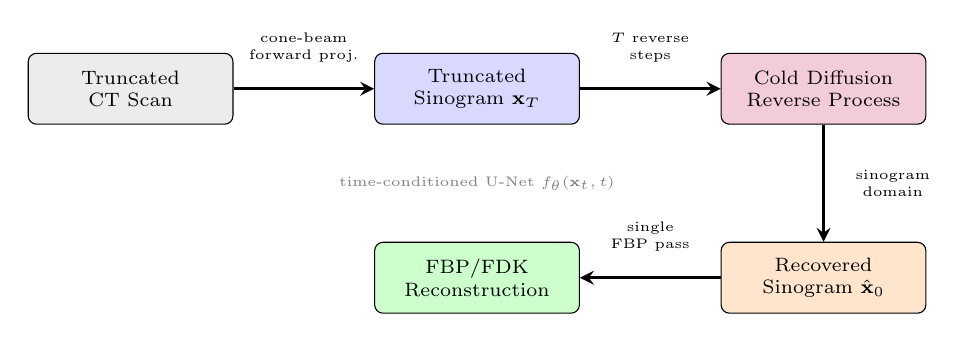
\begin{tikzpicture}[
  stage/.style={draw, rounded corners=3pt, minimum width=2.6cm, minimum height=0.9cm,
                font=\scriptsize, align=center, fill=#1},
  arr/.style={->, very thick, >=stealth},
  lbl/.style={font=\tiny, align=center, fill=white, inner sep=2pt, text depth=0pt},
]
%% Top row: acquisition  -->  truncated sinogram  -->  diffusion reverse
\node[stage=gray!15]    (scan)  at (0,0)    {Truncated\\CT Scan};
\node[stage=blue!15]    (sino)  at (4.4,0)  {Truncated\\Sinogram $\mathbf{x}_T$};
\node[stage=purple!20]  (diff)  at (8.8,0)  {Cold Diffusion\\Reverse Process};

%% Bottom row (snake): recovered sinogram  -->  FBP reconstruction
\node[stage=orange!20]  (rec)   at (8.8,-2.4) {Recovered\\Sinogram $\hat{\mathbf{x}}_0$};
\node[stage=green!20]   (fbp)   at (4.4,-2.4) {FBP/FDK\\Reconstruction};

%% Arrows
\draw[arr] (scan) -- node[above,lbl,yshift=8pt]{cone-beam\\forward proj.} (sino);
\draw[arr] (sino) -- node[above,lbl,yshift=8pt]{$T$ reverse\\steps} (diff);
\draw[arr] (diff) -- node[right,lbl,xshift=9pt]{sinogram\\domain} (rec);
\draw[arr] (rec)  -- node[above,lbl,yshift=8pt]{single\\FBP pass} (fbp);

%% Annotation
\node[font=\tiny, text=gray, align=center] at (4.4,-1.2)
  {time-conditioned U-Net\ $f_\theta(\mathbf{x}_t, t)$};

\end{tikzpicture}
}
\caption{System pipeline. A truncated CT acquisition is mapped to a sinogram via cone-beam forward projection. The Cold Diffusion reverse process iteratively recovers the missing detector columns through $T$ steps of a time-conditioned U-Net. The recovered sinogram is then reconstructed into an image using a single FBP/FDK pass.}
\label{fig:intro_pipeline_overview}
\end{figure}

\section{Thesis Structure}

The remainder of this thesis is organized as follows:

\textbf{Chapter~\ref{ch:background}} provides the necessary background on \gls{ct} imaging principles, truncation artifacts, and the mathematical foundations of the Radon transform and \gls{fbp} reconstruction.

\textbf{Chapter~\ref{ch:related_work}} reviews related work in truncation artifact correction, deep learning for medical imaging, and diffusion models for image restoration.

\textbf{Chapter~\ref{ch:methodology}} presents the core methodology of Cold Diffusion for sinogram-based field-of-view extension, including the forward degradation process, reverse generation process, and training objectives.

\textbf{Chapter~\ref{ch:experiments}} details the experimental design, datasets, baseline methods, and ablation study protocols.

\textbf{Chapter~\ref{ch:results}} describes the evaluation methodology and presents the quantitative and qualitative findings.

\textbf{Chapter~\ref{ch:discussion}} discusses the methodology, analyzes the approach's potential advantages and limitations, and compares it with existing methods.

\textbf{Chapter~\ref{ch:conclusion}} concludes the thesis and outlines future research directions.

\textbf{Appendix~A} documents the end-to-end data processing chain, including CT volume loading, cone-beam forward projection, normalization statistics, data organization, and quality-control checks.
